% Created 2021-10-29 Fri 20:57
\documentclass[9pt, b5paaper]{book}
\usepackage[UTF8]{ctex}
\usepackage{xltxtra}
\usepackage{bera}
\usepackage[T1]{fontenc}
\usepackage[scaled]{beraserif}
\usepackage[scaled]{berasans}
\usepackage[scaled]{beramono}
\usepackage{graphicx}
\usepackage{xcolor}
\usepackage{multirow}
\usepackage{multicol}
\usepackage{float}
\usepackage{textcomp}
\usepackage{geometry}
\geometry{left=1.2cm,right=1.2cm,top=1.5cm,bottom=1.2cm}
\usepackage{algorithm}
\usepackage{algorithmic}
\usepackage{latexsym}
\usepackage{natbib}
\usepackage{minted}
\newminted{common-lisp}{fontsize=ootnotesize}
\usepackage[xetex,colorlinks=true,CJKbookmarks=true,linkcolor=blue,urlcolor=blue,menucolor=blue]{hyperref}
\author{deepwaterooo}
\date{\today}
\title{plan}
\hypersetup{
  pdfkeywords={},
  pdfsubject={},
  pdfcreator={Emacs 27.1 (Org mode 8.2.7c)}}
\begin{document}

\maketitle
\tableofcontents


\chapter{Weekly Plan}
\label{sec-1}
\section{总结题型}
\label{sec-1-1}
\begin{itemize}
\item 我可能有一点儿傻做题,而不太懂得总结与作笔记。所以在现在刷得已经差不多,我需要更多的时间花在巩固与总结题型,把做题的经历真正转化为解题的分析能力。所以接下来一两周可能会对重要题型作相关的分析与总结,希望能够显著提升我做题和比赛中的解题命中率。

\item 这周刷得跟上一周差不多。计划接下来几周,每天刷10个题左右,一周60-70个题目,边刷边记错题进小本,到接下来的周六刷到1150左右;
\item dynamic programming, graph, segment tree等等剩下来的题目都是高难度的精华,需要好好练习和消化

\item 这个周主要复习了基础的部分,hashing, hashtable string two pointers, 以前很讨厌字符串,这个周写字符串看来,感觉基础的只要自己能够想得清楚的,都能很快实现出来,写得还比较得心应手。TreeMap, TreeSet也用得比较顺一点儿了
\item 写树的题目,dfs, bfs graph各种node,现在也是写得很顺心了,只是通过不断地测试加强巩固

\item 完成打基础的部分: hashing, hashmap, string, two pointer, sliding window,这些基础部分的题目,希望扫完
\item 如果某天头脑比较清醒、精力比较好的时候,会试图去慢速解决自己平时困难的地方:动态规划/ hashmap/hashing中数数组的个数,不常用的算法等

\item 数组相关的 segemnt tree, binary index tree等的基础,希望能够理解得再彻底一些,到能活学活用的程度
\item Deque双端队列O(n)解法的概念在建立,还需要很多的练习和熟悉
\item 最讨厌扫描线,几个双数怎么也数不清楚 heap等。。。。。。这个周扫几个出去

\item 如果说以前是迷迷糊糊刷题求AC,现在基本的概念在建立,希望从以前代码和题目的算法效率向代码优化中等偏优,寻求高效、最优解法的提升
\item bit manipulation, bitmasks基础知识基本掌握,还剩几道难题take my time慢慢解(感觉现在对bit操作,相对自信得心应手得多了!)
\item union find 的几个题,基本算是基本扫完吧,剩下的几下慢慢写。。。。。。

\item 很喜欢现在自己搭建出来的window刷题环境:WSL system, Zsh power shell, emacs configurations, locally everything, except Leetcode server is too slow, have to tolerant its latency\ldots{}\ldots{}

\item 至昨天晚上我终于意识到确定右侧单耳耳鸣,搬到现居住处后发病的(感觉现居住处到处都是电磁波干扰、洗衣烘衣的车床,厨房的冰箱,曾整小时整小时开过的洗手间风扇等),已经有几个周了。对于自2013年秋天野鸡大学的住宿环境以来,备受各种居住环境的困扰,尤其是2019年9月10月以来,我自小的听力受损,现在单侧耳鸣,可能的原因有家族遗传性高血压、遗传性脑血管肿瘤(外公舅舅和妈妈都受此脑溢血困扰过,大我五岁的亲姐姐前几个月也刚发此重病一次)等等。今天在网上稍搜索了一下相关信息,回想这几年的居住环境噪音和人为打扰与睡眠干扰、心里戚戚很不是滋味,希望我不至于会失去听力。
\item But my suffering is still only my/a personal suffering. Unless I could find an appropriate job, nobody cares if you are sick or not.因此,自信是本能,向往强大也是一种本能的向往。Anything happens, 我还是必须努力努力刷题,直到找到合适的工作.所以会近几周把剩下的一点儿题目刷完(hard and medium only, keep easy untouched dont care)不喜欢数字,也数字无缘,不打算写数组题目,如果一定要写,可能也只会把难题写一写吧
\end{itemize}

\section{比赛}
\label{sec-1-2}
\begin{itemize}
\item 会尽量多参加一些比赛,比赛时的效率还是相对好一点儿,所以每周一次、每半月一次,以及以后codeforces上的比赛,希望都能够尽量地多参加一些。
\end{itemize}

\section{数据规模与算法}
\label{sec-1-3}
\begin{center}
\begin{tabular}{rl}
\hline
Input Size & Complexity\\
\hline
50000 & O(n)\\
20000 & O(n logn)\\
\hline
1000 & O(n \^{} 2)\\
30 & O(n \^{} 4)\\
16 (20) & O(2 \^{} n)\\
\hline
\end{tabular}
\end{center}


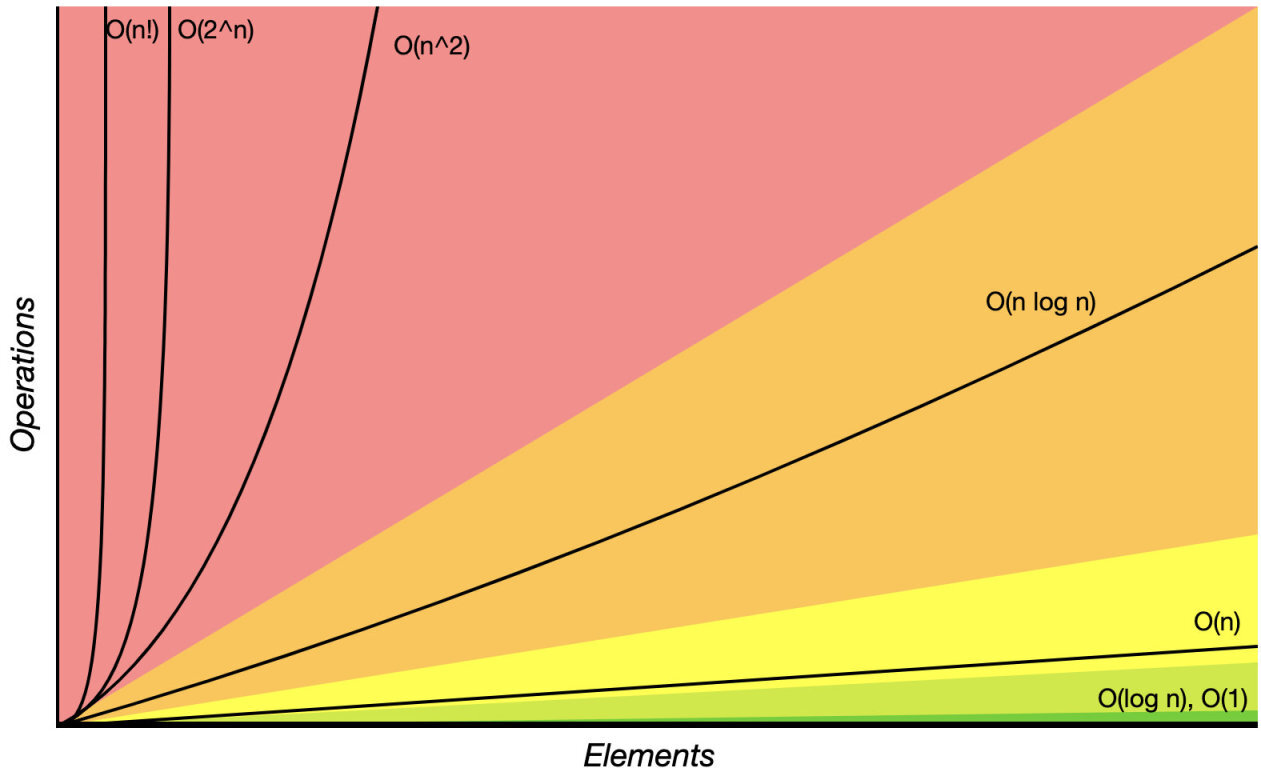
\includegraphics[width=.9\linewidth]{./pic/bigo.jpeg}

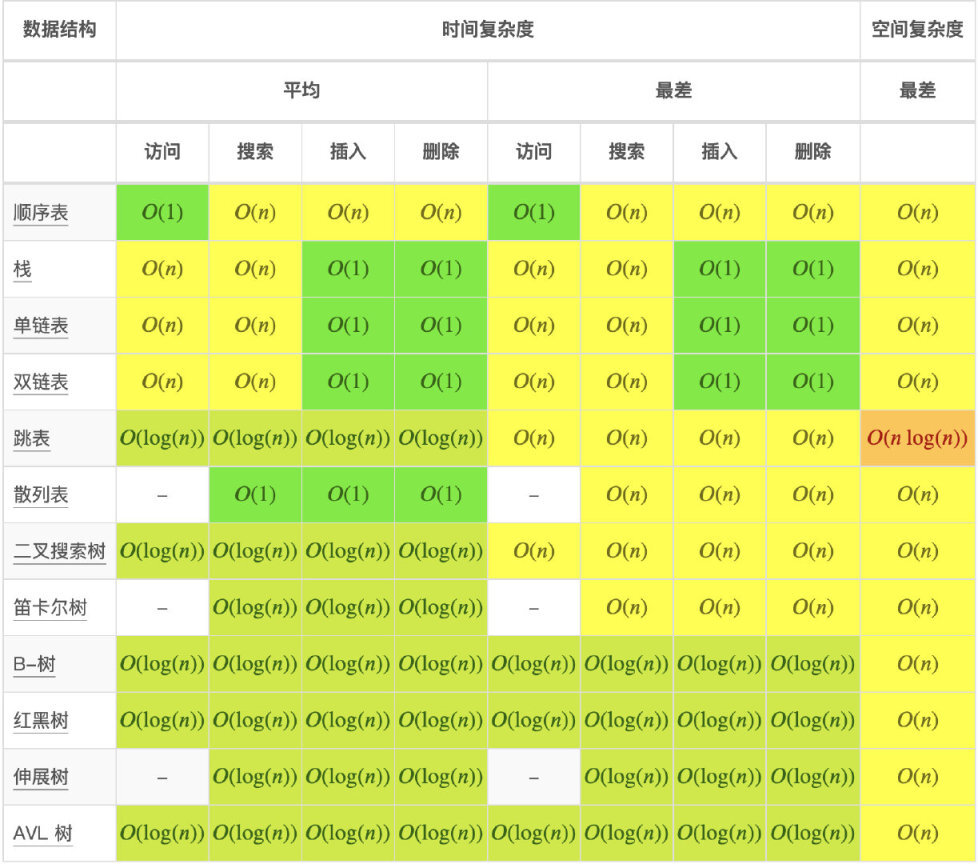
\includegraphics[width=.9\linewidth]{./pic/bigo2.jpeg}

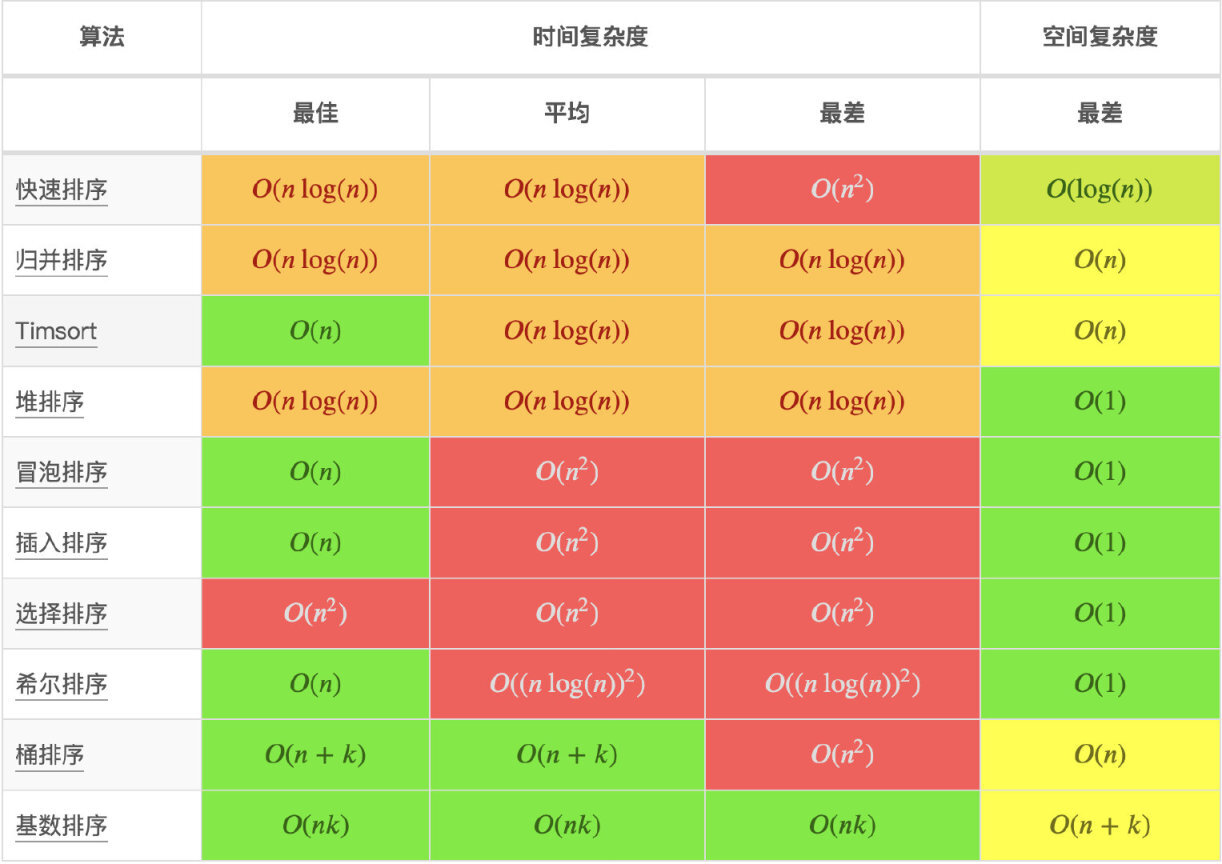
\includegraphics[width=.9\linewidth]{./pic/bigo3.jpeg}

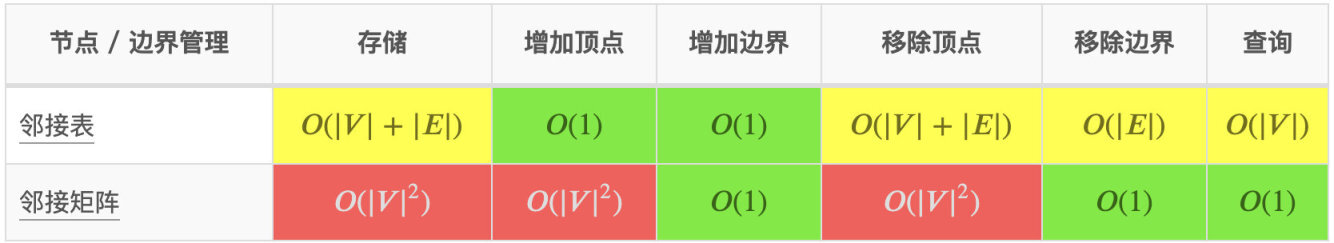
\includegraphics[width=.9\linewidth]{./pic/bigo4.jpeg}

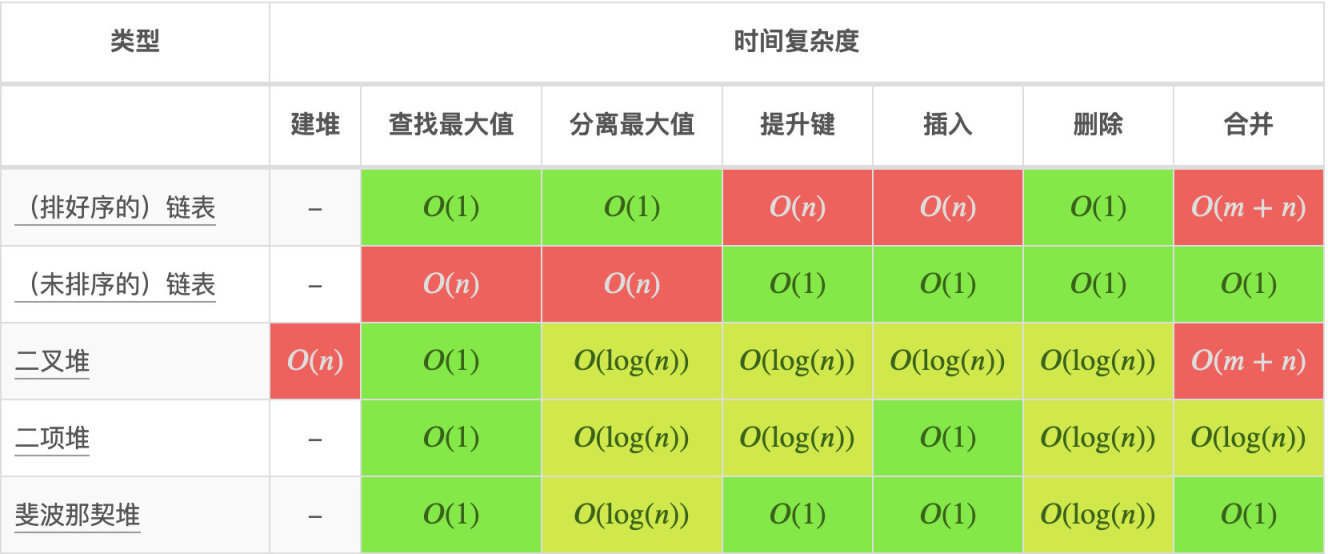
\includegraphics[width=.9\linewidth]{./pic/bigo5.jpeg}
% Emacs 27.1 (Org mode 8.2.7c)
\end{document}